\documentclass[
11pt, % The default document font size, options: 10pt, 11pt, 12pt
%codirector, % Uncomment to add a codirector to the title page
]{charter}
\usepackage{tikz}
\usetikzlibrary{positioning}




% El títulos de la memoria, se usa en la carátula y se puede usar el cualquier lugar del documento con el comando \ttitle
\titulo{Sistema de detección de interrupciones para subestaciones transformadoras de distribución de baja tensión}

% Nombre del posgrado, se usa en la carátula y se puede usar el cualquier lugar del documento con el comando \degreename
\posgrado{Carrera de Especialización en Sistemas Embebidos} 
%\posgrado{Carrera de Especialización en Internet de las Cosas} 
%\posgrado{Carrera de Especialización en Intelegencia Artificial}
%\posgrado{Maestría en Sistemas Embebidos} 
%\posgrado{Maestría en Internet de las cosas}

% Tu nombre, se puede usar el cualquier lugar del documento con el comando \authorname
\autor{Ing. Lucas Gabriel Robles}

% El nombre del director y co-director, se puede usar el cualquier lugar del documento con el comando \supname y \cosupname y \pertesupname y \pertecosupname
\director{Mg. Ing. Leonardo Del Sancio}
\pertenenciaDirector{FIUBA} 
% FIXME:NO IMPLEMENTADO EL CODIRECTOR ni su pertenencia
\codirector{John Doe} % para que aparezca en la portada se debe descomentar la opción codirector en el documentclass
\pertenenciaCoDirector{FIUBA}

% Nombre del cliente, quien va a aprobar los resultados del proyecto, se puede usar con el comando \clientename y \empclientename
\cliente{Ing. Adrián Abella}
\empresaCliente{EDET SA}

% Nombre y pertenencia de los jurados, se pueden usar el cualquier lugar del documento con el comando \jurunoname, \jurdosname y \jurtresname y \perteunoname, \pertedosname y \pertetresname.
\juradoUno{Nombre y Apellido (1)}
\pertenenciaJurUno{pertenencia (1)} 
\juradoDos{Nombre y Apellido (2)}
\pertenenciaJurDos{pertenencia (2)}
\juradoTres{Nombre y Apellido (3)}
\pertenenciaJurTres{pertenencia (3)}
 
\fechaINICIO{20 de octubre de 2022}		%Fecha de inicio de la cursada de GdP \fechaInicioName
\fechaFINALPlan{8 de diciembre de 2022} 	%Fecha de final de cursada de GdP
\fechaFINALTrabajo{a confirmar}	%Fecha de defensa pública del trabajo final


\begin{document}
\shorthandoff{>}
\shorthandoff{<}

\maketitle
\thispagestyle{empty}
\pagebreak


\thispagestyle{empty}
{\setlength{\parskip}{0pt}
\tableofcontents{}
}
\pagebreak


\section*{Registros de cambios}
\label{sec:registro}


\begin{table}[ht]
\label{tab:registro}
\centering
\begin{tabularx}{\linewidth}{@{}|c|X|c|@{}}
\hline
\rowcolor[HTML]{C0C0C0} 
Revisión & \multicolumn{1}{c|}{\cellcolor[HTML]{C0C0C0}Detalles de los cambios realizados} & Fecha      \\ \hline
0		& Creación del documento                                 &\fechaInicioName \\ \hline
1		& Redacción del acta de constitución del proyecto \newline
		Redacción de la descripción técnica-conceptual \newline
		Identificación y análisis de los interesados \newline
		Definición del propósito y alcance del proyecto
		& 3 de noviembre de 2022 \\ \hline
%2      & Se completa hasta el punto 7 inclusive
%		  Se puede agregar algo más \newline
%		  En distintas líneas \newline
%		  Así                                                    & dd/mm/aaaa \\ \hline
%3      & Se completa hasta el punto 11 inclusive                & dd/mm/aaaa \\ \hline
%4      & Se completa el plan	                                 & dd/mm/aaaa \\ \hline
\end{tabularx}
\end{table}

\pagebreak



\section*{Acta de constitución del proyecto}
\label{sec:acta}

\begin{flushright}
Buenos Aires, \fechaInicioName
\end{flushright}

\vspace{2cm}

Por medio de la presente se acuerda con el \authorname\hspace{1px} que su Trabajo Final de la \degreename\hspace{1px} se titulará ``\ttitle'', consistirá esencialmente en una red de sensores inalámbricos que detecten la ausencia de tensión y/o corriente en una subestación transformadora de distribución de baja tensión, y tendrá un presupuesto preliminar estimado de 600 hs de trabajo, con fecha de inicio \fechaInicioName\hspace{1px} y fecha de presentación pública \fechaFinalName.

Se adjunta a esta acta la planificación inicial.

\vfill

% Esta parte se construye sola con la información que hayan cargado en el preámbulo del documento y no debe modificarla
\begin{table}[ht]
\centering
\begin{tabular}{ccc}
\begin{tabular}[c]{@{}c@{}}Dr. Ing. Ariel Lutenberg \\ Director posgrado FIUBA\end{tabular} & \hspace{2cm} & \begin{tabular}[c]{@{}c@{}}\clientename \\ \empclientename \end{tabular} \vspace{2.5cm} \\ 
\multicolumn{3}{c}{\begin{tabular}[c]{@{}c@{}} \supname \\ Director del Trabajo Final\end{tabular}} \vspace{2.5cm} \\
%\begin{tabular}[c]{@{}c@{}}\jurunoname \\ Jurado del Trabajo Final\end{tabular}     &  & \begin{tabular}[c]{@{}c@{}}\jurdosname\\ Jurado del Trabajo Final\end{tabular}  \vspace{2.5cm}  \\
%\multicolumn{3}{c}{\begin{tabular}[c]{@{}c@{}} \jurtresname\\ Jurado del Trabajo Final\end{tabular}} \vspace{.5cm}                                                                     
\end{tabular}
\end{table}




\section{1. Descripción técnica-conceptual del proyecto a realizar}
\label{sec:descripcion}

Uno de los principales objetivos de una empresa de distribución eléctrica es mantener los índices de calidad de servicio y producto técnico dentro de determinados parámetros predefinidos para garantizar que el usuario final goce de una buena calidad de suministro eléctrico. Es por esta razón que la gestión de la calidad de producto técnico se ocupa de que la onda de tensión suministrada se encuentre dentro de los umbrales establecidos por la entidad reguladora, mientras que la gestión de la calidad de servicio técnico se encarga de minimizar el tiempo y la frecuencia de las interrupciones del suministro eléctrico.
Gracias al avance tecnológico, se pudieron adoptar nuevos sistemas capaces de optimizar la gestión de reclamos por falta de suministro, lo que permitió agilizar el proceso de restablecimiento del servicio y, por consiguiente, aminorar el tiempo en el que un cliente se encuentra desenergizado. A pesar de ello, estos sistemas pueden carecer de precisión al momento de determinar las posibles causas y las zonas afectadas por la interrupción, lo que en ocasiones resulta en una mala gestión de los recursos y las tareas. Por lo expuesto, se le propone a la Empresa de Distribución Eléctrica de Tucumán (EDET SA) implementar la utilización de un sistema electrónico embebido que sea capaz de sensar a nivel de cada subestación transformadora de baja tensión el estado del suministro eléctrico. Esto permitirá, en caso de ocurrir una interrupción, detectarla inmediatamente y así poder contar con una mayor velocidad de respuesta, mayor precisión, menor tiempo de reposición del servicio y menor cantidad de personal abocado a estas tareas. En la Figura 1 se muestra el diagrama en bloques del sistema propuesto, en el que se pueden diferenciar dos componentes principales: el nodo sensor (izquierda) y el concentrador o \textit{Gateway} (derecha).

\begin{figure}[htpb]
\centering 
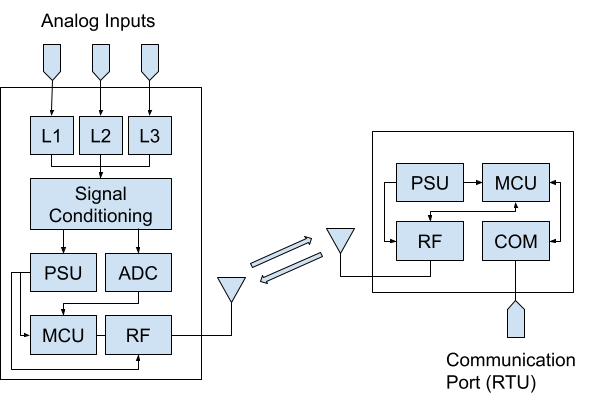
\includegraphics[width=.7\textwidth]{./Figuras/image1.png}
\caption{Diagrama en bloques del sistema.}
\label{fig:diagBloques}
\end{figure}

El concentrador o \textit{Gateway} será el encargado de gestionar y monitorear la red de nodos sensores y de almacenar la información que luego será consultada por la \textit{RTU}. Estará conformado por un microcontrolador de 32 bits, una fuente de alimentación que puede adicionalmente funcionar como cargador de baterías, un módulo de conectividad inalámbrica mediante el cual se comunicará con los nodos sensores y un puerto de comunicaciones para la conexión con la \textit{RTU}. 
Respecto al módulo RF, en principio se propone utilizar alguna tecnología \textit{LPWAN }(\textit{Low Power Wide Area Network}) para minimizar el consumo de energía y proporcionar un largo alcance. En cuanto a las comunicaciones con la unidad remota, se propone utilizar el protocolo Modbus-RTU o Modbus-TCP.
Los nodos sensores serán los encargados de traducir las variables analógicas (tensiones y/o corrientes) en señales digitales binarias \textit{ON-OFF} que se activarán si se superan los umbrales predefinidos; luego, estas serán transmitidas hacia el concentrador. Se propone que sea de esta manera para minimizar la cantidad de información enviada, lo que permitirá ahorrar espacio de almacenamiento, reducir la cantidad de información transmitida hacia el sistema SCADA y reducir los tiempos de actualización de los estados y las alarmas. También se prevé que cada nodo sensor posea una fuente de alimentación capaz de obtener su energía sin necesidad de conectarla a la red de 220 V, siendo las opciones más probables las que operen con energía solar o inducción magnética. La intención de esta prestación es la de facilitar la instalación del sistema, además de reducir el riesgo eléctrico al eliminar la necesidad de conectarse directamente a la red de baja tensión.
Al igual que el concentrador, los nodos también contarán con un microcontrolador de 32 bits, aunque se espera que estos sean de baja potencia o que admitan trabajar en modos de ultra bajo consumo o \textit{deep-sleep}. También se utilizarán los mismos módulos RF \textit{LPWAN} para la comunicación con el \textit{Gateway}.


\section{2. Identificación y análisis de los interesados}
\label{sec:interesados}

\begin{table}[ht]
%\caption{Identificación de los interesados}
%\label{tab:interesados}
\begin{tabularx}{\linewidth}{@{}|l|X|X|l|@{}}
\hline
\rowcolor[HTML]{C0C0C0} 
Rol           & Nombre y Apellido & Organización 	& Puesto 	\\ \hline
%Auspiciante  &                   &              	&        	\\ \hline
Cliente       & \clientename      &\empclientename	& Jefe de Calidad de Servicio \\ \hline
%Impulsor     &                   &              	&        	\\ \hline
Responsable   & \authorname       & FIUBA        	& Alumno 	\\ \hline
%Colaboradores&                   &              	&        	\\ \hline
Orientador    & \supname	      & \pertesupname 	& Director Trabajo Final \\ \hline
%Equipo       & miembro1 \newline 
%				miembro2          &              	&        	\\ \hline
%Opositores   &                   &              	&        	\\ \hline
Usuario final &       EDET SA     &              	&        	\\ \hline
\end{tabularx}
\end{table}



\section{3. Propósito del proyecto}
\label{sec:proposito}

Mejora de la calidad del servicio eléctrico brindado por la distribuidora mediante la obtención de información precisa y en tiempo real sobre el estado del suministro eléctrico en subestaciones transformadoras (SETS) de baja tensión a través de un sistema distribuido de sensores inalámbricos que detecten la presencia de tensión y/o corriente en cada una de las salidas de baja tensión de las SETS.

\section{4. Alcance del proyecto}
\label{sec:alcance}

Se encuentra dentro del alcance de este proyecto el desarrollo del hardware y del firmware de ambos componentes principales: concentrador y nodo sensor. Se espera desarrollar al menos una unidad del primero y al menos dos del segundo. Los nodos sensores deberán ser capaces de convertir las señales analógicas de tensión y/o corriente en señales digitales binarias y transmitirlas hacia el concentrador. El concentrador deberá ser capaz de recibir la información enviada por los nodos sensores, almacenarla en una memoria no volátil y organizarla de acuerdo con las especificaciones del protocolo Modbus. También deberá proveer un método o interfaz que le permita a una unidad terminal remota acceder a dicha información.

No se incluye en el desarrollo del proyecto la encriptación de la información transmitida desde los sensores hacia el concentrador. Tampoco se incluye el desarrollo de una interfaz humano-máquina (HMI) para la configuración de los dispositivos y la visualización de la información.


\section{5. Supuestos del proyecto}
\label{sec:supuestos}

Para el desarrollo del presente proyecto se supone que:

\begin{itemize}
	\item Se podrá adquirir todos los componentes necesarios para el desarrollo de los dispositivos.
	\item Se podrán realizar pruebas de campo en instalaciones reales.
	\item Se podrá utilizar una unidad de transmisión remota de la distribuidora para enviar la información al sistema SCADA.
	\item Se podrán dedicar al menos 15 horas semanales al desarrollo del proyecto.
	\item Se podrá finalizar el proyecto en 600 horas o menos.
\end{itemize}

\section{6. Requerimientos}
\label{sec:requerimientos}

\begin{enumerate}
	\item Requerimientos funcionales
		\begin{enumerate}
			\item Los dispositivos deben ser de tipo \textit{Plug and Play}.
			\item La distancia mínima de comunicación entre los nodos y el \textit{Gateway} debe ser de 3 metros.
			\item El emparejamiento entre los nodos y el \textit{Gateway} debe ser automático.
			\item Tanto el \textit{Gateway} como los nodos sensores deben almacenar la información de la red en memoria no volátil.
			\item Los nodos sensores deben enviar el estado del suministro eléctrico cada 1 minuto.
		\end{enumerate}
	\item Requerimientos de hardware
		\begin{enumerate}
			\item El \textit{Gateway} debe estar basado en un microcontrolador ESP32 del fabricante Espressif.
			\item Cada nodo sensor debe estar basado en un microcontrolador ESP8266 del fabricante Espressif.
			\item El \textit{Gateway} debe contar con una fuente de alimentación universal de 220 VAC.
			\item Los nodos sensores deben poseer una fuente de alimentación que utilice energía solar o inducción magnética.
			\item Los nodos sensores deben poseer 3 entradas de corriente o tensión, las cuales:
				\begin{itemize}
					\item se deben conectar a la línea de baja tensión (220/380 VAC) por intermedio de transformadores de corriente o de tensión,
					\item deben soportar hasta 100 A o 1000 V en el lado primario,
					\item deben soportar hasta 1 A o 5 V en el lado secundario.
				\end{itemize}						
		\end{enumerate}
	\item Requerimientos de firmware
		\begin{enumerate}
			\item El firmware del \textit{Gateway} debe:
				\begin{itemize}
					\item administrar la red de nodos sensores y poseer un algoritmo para registrarlos y desvincularlos de esta,
					\item almacenar la información de cada uno de los nodos sensores registrados en la red,
					\item consultar el estado y las mediciones de los nodos sensores,
					\item almacenar la información obtenida de los sensores en una base de datos Modbus,
					\item proveer una interfaz de comunicación que permita que la base de datos sea consultada por una RTU.
				\end{itemize}
			\item El firmware de los nodos sensores debe:
				\begin{itemize}
					\item procesar las señales analógicas y convertirlas en señales digitales binarias \textit{ON-OFF} que indiquen el estado del suministro eléctrico,
					\item transmitir el estado del suministro hacia el \textit{Gateway} a través del módulo RF \textit{LPWAN},
					\item poner en modo de bajo consumo al microcontrolador y al módulo RF mientras no se esté transmitiendo información.
				\end{itemize}
		\end{enumerate}
\end{enumerate}


\section{7. Historias de usuarios (\textit{Product backlog})}
\label{sec:backlog}

Se analizan las historias de usuario con los índices de ponderación que representan el valor que
aporta la historia de usuario al cliente o usuario y con el índice de prioridad que refleja el orden
de importancia en la implementación de las historias. Se valora cada dimensión de 1 a 10, donde
10 representa la ponderación o prioridad más alta. Los \textit{story points} se calculan como la suma
de la ponderación y la prioridad.

Como encargado del área de calidad de servicio quiero conocer en tiempo real el estado del suministro eléctrico de cada subestación transformadora para reducir el tiempo en el que los usuarios se encuentran sin suministro.

\begin{itemize}
	\item Ponderación: 10.
	\item Prioridad: 8.
	\item \textit{Story Points:} 18.
\end{itemize}

Como encargado del área de operaciones quiero conocer en todo momento el estado de la red de distribución para poder contar con mayor información posible a la hora de realizar las operaciones.

\begin{itemize}
	\item Ponderación: 6.
	\item Prioridad: 5.
	\item \textit{Story Points:} 11.
\end{itemize}

Como encargado del área de reclamos quiero conocer de manera inequívoca e inmediata las zonas que se encuentran afectadas por un corte de energía para poder gestionar eficientemente los recursos humanos con los que contamos.

\begin{itemize}
	\item Ponderación: 9.
	\item Prioridad: 7.
	\item \textit{Story Points:} 16.
\end{itemize}

Como encargado del área de mantenimiento de la red quiero conocer cuáles son las subestaciones transformadoras o las zonas con mayor tasa de fallas para realizar un mejor plan de mantenimiento y enfocar las inversiones en esos lugares.

\begin{itemize}
	\item Ponderación: 5.
	\item Prioridad: 4.
	\item \textit{Story Points:} 9.
\end{itemize}

\section{8. Entregables principales del proyecto}
\label{sec:entregables}

Los entregables del proyecto son:

\begin{itemize}
	\item Un prototipo de \textit{Gateway}.
	\item Dos prototipos de nodo sensor.
	\item Manual de uso.
	\item Diagrama de instalación.
	\item Listado de materiales.
	\item Diagramas esquemáticos.
	\item Informe final.
\end{itemize}

\section{9. Desglose del trabajo en tareas}
\label{sec:wbs}


\begin{enumerate}
\item Gestión y documentación (220 horas).
	\begin{enumerate}
	\item Planificación del proyecto (40 horas).
	\item Investigación preliminar (20 horas).
	\item Documentación de avances (20 horas).
	\item Confección de la memoria técnica (80 horas).
	\item Elaboración de la presentación final (20 horas).
	\item Redacción del manual de usuario (40 horas).
	\end{enumerate}
\item Desarrollo de hardware (210 horas).
	\begin{enumerate}
	\item Diseño preliminar (20 horas).
	\item Diseño de esquemáticos del \textit{Gateway} (20 horas).
	\item Diseño de esquemáticos del nodo sensor (20 horas).
	\item Construcción de prototipo del \textit{Gateway} (40 horas).
	\item Construcción de prototipo del nodo sensor (40 horas).
	\item Diseño de PCB (20 horas).
	\item Fabricación de PCB (20 horas).
	\item Compra de componentes (10 horas).
	\item Armado de PCB (20 horas).
	\end{enumerate}
\item Desarrollo de firmware (130 horas).
	\begin{enumerate}
	\item Diseño preliminar (20 horas).
	\item Desarrollo del código para el \textit{Gateway} (40 horas).
	\item Desarrollo del código para el nodo sensor (40 horas).
	\item Pruebas de funcionamiento (30 horas).
	\end{enumerate}
\item Verificación y finalización (40 horas).
	\begin{enumerate}
	\item Montaje final (20 horas).
	\item Pruebas funcionales (20 horas).
	\end{enumerate}
\end{enumerate}

Cantidad total de horas: 600.

%\begin{landscape}
\section{10. Diagrama de Activity On Node}
\label{sec:AoN}

En la Figura 2 se observa el diagrama de \textit{Activity on Node} con los tiempos en horas de trabajo.
El camino critico se encuentra resaltado con trazo grueso, en el que se totalizan 390 horas.
\\

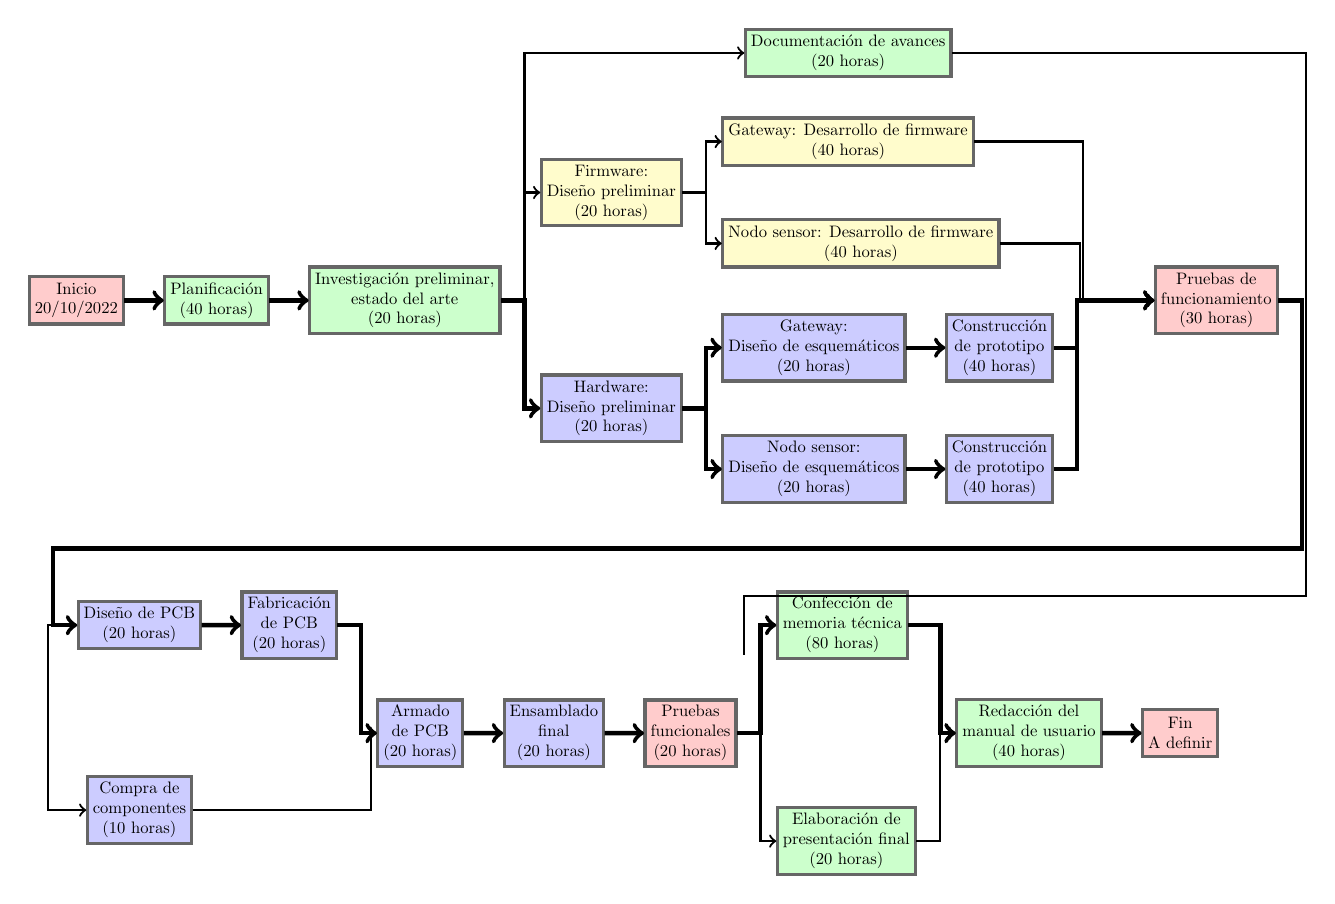
\begin{tikzpicture}[
hito/.style={rectangle, draw=black!60, fill=red!20, very thick, minimum size=10mm, scale=0.6, align=center},
plan/.style={rectangle, draw=black!60, fill=green!20, very thick, minimum size=10mm, scale=0.6, align=center},
hw/.style={rectangle, draw=black!60, fill=blue!20, very thick, minimum size=10mm, scale=0.6, align=center},
fw/.style={rectangle, draw=black!60, fill=yellow!20, very thick, minimum size=10mm, scale=0.6, align=center},
scale=3
]
%Nodes
\node[hito]	(iniciar)																{Inicio\\ 20/10/2022};
\node[plan]	(planificar)		[right= 0.5cm of iniciar]							{Planificación\\ (40 horas)};
\node[plan]	(investigar)	 	[right= 0.5cm of planificar]						{Investigación preliminar,\\ estado del arte\\ (20 horas)};
\node[fw]	(firmware_pre)	 	[above right= 0.5cm and 0.5cm of investigar]		{Firmware:\\ Diseño preliminar\\ (20 horas)};
\node[hw]	(hardware_pre)	 	[below right= 0.5cm and 0.5cm of investigar]		{Hardware:\\ Diseño preliminar\\ (20 horas)};
\node[fw]	(firmware_gw_dis)	[above right= -0.1cm and 0.5cm of firmware_pre]		{Gateway: Desarrollo de firmware\\ (40 horas)};
\node[fw]	(firmware_nodo_dis)	[below right= -0.1cm and 0.5cm of firmware_pre]		{Nodo sensor: Desarrollo de firmware\\ (40 horas)};
\node[hw]	(hardware_gw_dis)	[above right= -0.1cm and 0.5cm of hardware_pre]		{Gateway:\\ Diseño de esquemáticos\\ (20 horas)};
\node[hw] 	(hardware_nodo_dis)	[below right= -0.1cm and 0.5cm of hardware_pre]		{Nodo sensor:\\ Diseño de esquemáticos\\ (20 horas)};
\node[hw] 	(hardware_gw_prot)	[right= 0.5cm of hardware_gw_dis]					{Construcción\\ de prototipo\\ (40 horas)};
\node[hw] 	(hardware_nodo_prot)[right= 0.5cm of hardware_nodo_dis]					{Construcción\\ de prototipo\\ (40 horas)};
\node[hito] (firmware_test)		[right= 8.3cm of investigar]						{Pruebas de\\ funcionamiento\\ (30 horas)};
\node[hw] 	(hardware_pcb_dis)	[below right= 3.5cm and -0.6cm of iniciar]			{Diseño de PCB\\ (20 horas)};
\node[hw] 	(hardware_comp_buy)	[below= 1.6cm of hardware_pcb_dis]					{Compra de\\ componentes\\ (10 horas)};
\node[hw] 	(hardware_pcb_make)	[right= 0.5cm of hardware_pcb_dis]					{Fabricación\\ de PCB\\ (20 horas)};
\node[hw] 	(hardware_pcb_asm)	[below right= 0.5cm and 0.5cm of hardware_pcb_make]	{Armado\\ de PCB\\ (20 horas)};
\node[hw] 	(final_assembly)	[right= 0.5cm of hardware_pcb_asm]						{Ensamblado\\ final\\ (20 horas)};
\node[hito]	(final_test)		[right= 0.5cm of final_assembly]					{Pruebas\\ funcionales\\ (20 horas)};
\node[plan]	(progress_doc)		[above= 0.5cm of firmware_gw_dis]					{Documentación de avances\\ (20 horas)};
\node[plan] (tech_mem_make)		[above right= 0.5cm and 0.5cm of final_test]		{Confección de\\ memoria técnica\\ (80 horas)};
\node[plan] (presentation_make)	[below right= 0.5cm and 0.5cm of final_test]		{Elaboración de\\ presentación final\\ (20 horas)};
\node[plan] (user_manual_make)	[above right= 0.5cm and 0.5cm of presentation_make]	{Redacción del\\ manual de usuario\\ (40 horas)};
\node[hito]	(finalizar)			[right= 0.5cm of user_manual_make]					{Fin\\ A definir};

%Lines
\draw[ultra thick, ->] (iniciar.east)			-- 					(planificar.west);
\draw[ultra thick, ->] (planificar.east)		-- 					(investigar.west);
\draw[thick, ->] (investigar.east)				--	+(0.1,0)	|-	(firmware_pre.west);
\draw[ultra thick, ->] (investigar.east)		-- 	+(0.1,0)	|-	(hardware_pre.west);
\draw[thick, ->] (investigar.east)				--	+(0.1,0)	|-	(progress_doc.west);
\draw[thick, ->] (firmware_pre.east)			-- 	+(0.1,0)	|-	(firmware_gw_dis.west);
\draw[thick, ->] (firmware_pre.east)			-- 	+(0.1,0)	|-	(firmware_nodo_dis.west);
\draw[ultra thick, ->] (hardware_pre.east)		-- 	+(0.1,0)	|-	(hardware_gw_dis.west);
\draw[ultra thick, ->] (hardware_pre.east)		-- 	+(0.1,0)	|-	(hardware_nodo_dis.west);
\draw[thick, ->] (firmware_gw_dis.east)			-- 	+(0.46,0)	|-	(firmware_test);
\draw[thick, ->] (firmware_nodo_dis.east)		--	+(0.34,0)	|-	(firmware_test);
\draw[ultra thick, ->] (hardware_gw_dis.east)	--	+(0.1,0)	|-	(hardware_gw_prot.west);
\draw[ultra thick, ->] (hardware_nodo_dis.east)	--	+(0.1,0)	|-	(hardware_nodo_prot.west);
\draw[ultra thick, ->] (hardware_gw_prot.east)	--	+(0.1,0)	|-	(firmware_test.west);
\draw[ultra thick, ->] (hardware_nodo_prot.east)--	+(0.1,0)	|-	(firmware_test.west);
\draw[ultra thick, ->] (firmware_test.east)		--	+(0.1,0)	--	+(0.1,-1.05) -- (-0.1,-1.05) |- (hardware_pcb_dis.west);
\draw[thick, ->] (hardware_pcb_dis.west)		--	+(-0.123,0)	|-	(hardware_comp_buy.west);
\draw[ultra thick, ->] (hardware_pcb_dis.east)	--					(hardware_pcb_make.west);
\draw[ultra thick, ->] (hardware_pcb_make.east)	--	+(0.1,0)	|-	(hardware_pcb_asm.west);
\draw[thick, ->] (hardware_comp_buy.east)		--	+(0.755,0)	|-	(hardware_pcb_asm.west);
\draw[thick,  -] (progress_doc.east)			--	+(1.5,0)	--	+(1.5,-2.3)	--	+(-0.88,-2.3) -- +(-0.88, -2.55);
\draw[ultra thick, ->] (hardware_pcb_asm.east)	--					(final_assembly.west);
\draw[ultra thick, ->] (final_assembly.east)	--					(final_test.west);
\draw[ultra thick, ->] (final_test.east)		--	+(0.1,0)	|-	(tech_mem_make.west);
\draw[thick, ->] (final_test.east)				--	+(0.1,0)	|-	(presentation_make.west);
\draw[ultra thick, ->] (tech_mem_make.east)		--	+(0.135,0)	|-	(user_manual_make.west);
\draw[thick, ->] (presentation_make.east)		--	+(0.1,0)	|-	(user_manual_make.west);
\draw[ultra thick, ->] (user_manual_make.east)	--	+(0.1,0)	--	(finalizar.west);


\end{tikzpicture}
%\end{landscape}

\begin{landscape}
\section{11. Diagrama de Gantt}
\label{sec:gantt}

\begin{figure}[htpb]
\centering 
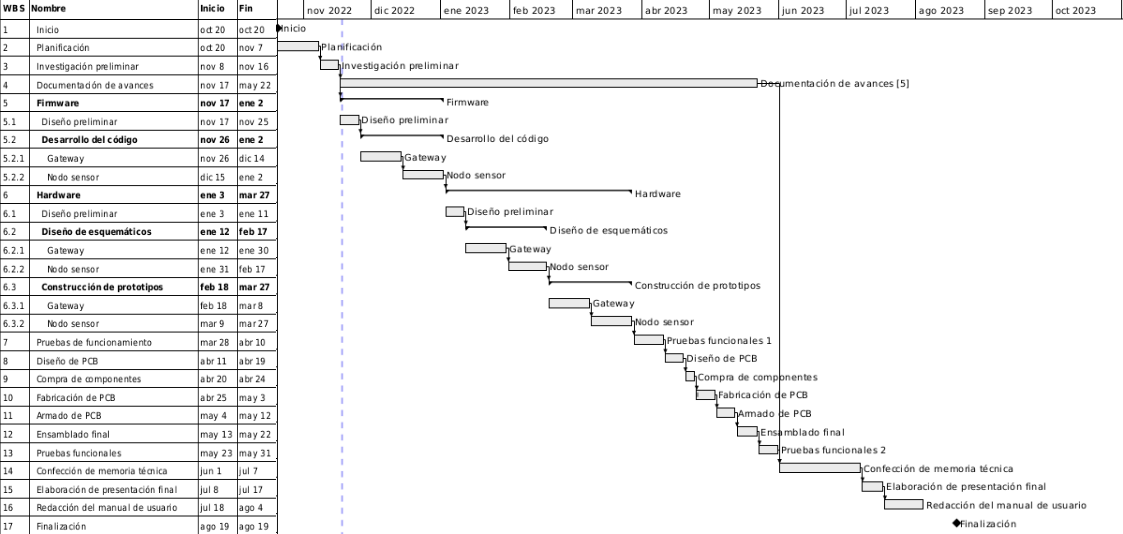
\includegraphics[height=.72\textheight]{./Figuras/Gantt.png}
\caption{Diagrama de Gantt}
\label{fig:diagGantt}
\end{figure}

\end{landscape}


\section{12. Presupuesto detallado del proyecto}
\label{sec:presupuesto}

\begin{table}[htpb]
\centering
\begin{tabularx}{\linewidth}{@{}|X|c|r|r|@{}}
\hline
\rowcolor[HTML]{C0C0C0} 
\multicolumn{4}{|c|}{\cellcolor[HTML]{C0C0C0}COSTOS DIRECTOS} \\ \hline
\rowcolor[HTML]{C0C0C0} 
Descripción &
  \multicolumn{1}{c|}{\cellcolor[HTML]{C0C0C0}Cantidad} &
  \multicolumn{1}{c|}{\cellcolor[HTML]{C0C0C0}Valor unitario (AR\$)} &
  \multicolumn{1}{c|}{\cellcolor[HTML]{C0C0C0}Valor total(AR\$)} \\ \hline
ESP32 Development Board &
  \multicolumn{1}{c|}{1} &
  \multicolumn{1}{c|}{4285} &
  \multicolumn{1}{c|}{4285} \\ \hline
ESP8266 Development Board &
  \multicolumn{1}{c|}{2} &
  \multicolumn{1}{c|}{2000} &
  \multicolumn{1}{c|}{4000} \\ \hline
SX1278 LoRa Module &
  \multicolumn{1}{c|}{3} &
  \multicolumn{1}{c|}{3542} &
  \multicolumn{1}{c|}{10626} \\ \hline
Sensor de corriente efecto Hall 100 A &
  \multicolumn{1}{c|}{3} &
  \multicolumn{1}{c|}{4415} &
  \multicolumn{1}{c|}{13245} \\ \hline
Batería de litio 18650 3,7 V &
  \multicolumn{1}{c|}{2} &
  \multicolumn{1}{c|}{2230} &
  \multicolumn{1}{c|}{4460} \\ \hline
Fabricación de PCB &
  \multicolumn{1}{c|}{3} &
  \multicolumn{1}{c|}{3000} &
  \multicolumn{1}{c|}{9000} \\ \hline
Resistencias, capacitores, conectores, etc &
  \multicolumn{1}{c|}{3} &
  \multicolumn{1}{c|}{1000} &
  \multicolumn{1}{c|}{3000} \\ \hline
Hora de trabajo &
  \multicolumn{1}{c|}{600} &
  \multicolumn{1}{c|}{2000} &
  \multicolumn{1}{c|}{1200000} \\ \hline
\multicolumn{3}{|c|}{SUBTOTAL} &
  \multicolumn{1}{c|}{1248616} \\ \hline
\rowcolor[HTML]{C0C0C0} 
\multicolumn{4}{|c|}{\cellcolor[HTML]{C0C0C0}COSTOS INDIRECTOS} \\ \hline
\rowcolor[HTML]{C0C0C0} 
Descripción &
  \multicolumn{1}{c|}{\cellcolor[HTML]{C0C0C0}Cantidad} &
  \multicolumn{1}{c|}{\cellcolor[HTML]{C0C0C0}Valor unitario} &
  \multicolumn{1}{c|}{\cellcolor[HTML]{C0C0C0}Valor total} \\ \hline
40\% de los costos directos &
  \multicolumn{1}{c|}{} &
  \multicolumn{1}{c|}{} &
  \multicolumn{1}{c|}{19449,40} \\ \hline

\multicolumn{3}{|c|}{SUBTOTAL} &
  \multicolumn{1}{c|}{19449,40} \\ \hline
\rowcolor[HTML]{C0C0C0}
\multicolumn{3}{|c|}{TOTAL} & 
\multicolumn{1}{c|}{1268062,40} \\ \hline
\end{tabularx}%
\end{table}


\section{13. Gestión de riesgos}
\label{sec:riesgos}

\begin{consigna}{red}
a) Identificación de los riesgos (al menos cinco) y estimación de sus consecuencias:
 
Riesgo 1: detallar el riesgo (riesgo es algo que si ocurre altera los planes previstos de forma negativa)
\begin{itemize}
	\item Severidad (S): mientras más severo, más alto es el número (usar números del 1 al 10).\\
	Justificar el motivo por el cual se asigna determinado número de severidad (S).
	\item Probabilidad de ocurrencia (O): mientras más probable, más alto es el número (usar del 1 al 10).\\
	Justificar el motivo por el cual se asigna determinado número de (O). 
\end{itemize}   

Riesgo 2:
\begin{itemize}
	\item Severidad (S): 
	\item Ocurrencia (O):
\end{itemize}

Riesgo 3:
\begin{itemize}
	\item Severidad (S): 
	\item Ocurrencia (O):
\end{itemize}


b) Tabla de gestión de riesgos:      (El RPN se calcula como RPN=SxO)

\begin{table}[htpb]
\centering
\begin{tabularx}{\linewidth}{@{}|X|c|c|c|c|c|c|@{}}
\hline
\rowcolor[HTML]{C0C0C0} 
Riesgo & S & O & RPN & S* & O* & RPN* \\ \hline
       &   &   &     &    &    &      \\ \hline
       &   &   &     &    &    &      \\ \hline
       &   &   &     &    &    &      \\ \hline
       &   &   &     &    &    &      \\ \hline
       &   &   &     &    &    &      \\ \hline
\end{tabularx}%
\end{table}

Criterio adoptado: 
Se tomarán medidas de mitigación en los riesgos cuyos números de RPN sean mayores a...

Nota: los valores marcados con (*) en la tabla corresponden luego de haber aplicado la mitigación.

c) Plan de mitigación de los riesgos que originalmente excedían el RPN máximo establecido:
 
Riesgo 1: plan de mitigación (si por el RPN fuera necesario elaborar un plan de mitigación).
  Nueva asignación de S y O, con su respectiva justificación:
  - Severidad (S): mientras más severo, más alto es el número (usar números del 1 al 10).
          Justificar el motivo por el cual se asigna determinado número de severidad (S).
  - Probabilidad de ocurrencia (O): mientras más probable, más alto es el número (usar del 1 al 10).
          Justificar el motivo por el cual se asigna determinado número de (O).

Riesgo 2: plan de mitigación (si por el RPN fuera necesario elaborar un plan de mitigación).
 
Riesgo 3: plan de mitigación (si por el RPN fuera necesario elaborar un plan de mitigación).

\end{consigna}


\section{14. Gestión de la calidad}
\label{sec:calidad}

\begin{consigna}{red}
Para cada uno de los requerimientos del proyecto indique:
\begin{itemize} 
\item Req \#1: copiar acá el requerimiento.

\begin{itemize}
	\item Verificación para confirmar si se cumplió con lo requerido antes de mostrar el sistema al cliente. Detallar 
	\item Validación con el cliente para confirmar que está de acuerdo en que se cumplió con lo requerido. Detallar  
\end{itemize}

\end{itemize}

Tener en cuenta que en este contexto se pueden mencionar simulaciones, cálculos, revisión de hojas de datos, consulta con expertos, mediciones, etc.  Las acciones de verificación suelen considerar al entregable como ``caja blanca'', es decir se conoce en profundidad su funcionamiento interno.  En cambio, las acciones de validación suelen considerar al entregable como ``caja negra'', es decir, que no se conocen los detalles de su funcionamiento interno.

\end{consigna}

\section{15. Procesos de cierre}    
\label{sec:cierre}

\begin{consigna}{red}
Establecer las pautas de trabajo para realizar una reunión final de evaluación del proyecto, tal que contemple las siguientes actividades:

\begin{itemize}
	\item Pautas de trabajo que se seguirán para analizar si se respetó el Plan de Proyecto original:
	 - Indicar quién se ocupará de hacer esto y cuál será el procedimiento a aplicar. 
	\item Identificación de las técnicas y procedimientos útiles e inútiles que se emplearon, y los problemas que surgieron y cómo se solucionaron:
	 - Indicar quién se ocupará de hacer esto y cuál será el procedimiento para dejar registro.
	\item Indicar quién organizará el acto de agradecimiento a todos los interesados, y en especial al equipo de trabajo y colaboradores:
	  - Indicar esto y quién financiará los gastos correspondientes.
\end{itemize}

\end{consigna}


\end{document}
